\chapter{Experiment} 
\label{Chapter3} 
\lhead{Chapter 3. \emph{Experiment}} 

\section{Client throughout}

\subsection{Client scalability}

SocketCluster-client makes the instanciation of a WebSocket clients on one core
quite straightforward. To deploy it on all available nodes, node.js
\texttt{fork()} function is used. A client code example is given in appendix
\ref{fig:WS_client_simplePing}.

The first experiment is a safety test. It checks if \texttt{fork()} distributes
evenly the work among the cores.

\begin{center}
  \begin{tabular}{ | l | l |}
  \hline
  \multicolumn{2}{|c|}{Parameters} \\
  \hline
    Instance type &  amazon s3 m3.2xlarge\\ 
    Experiment time & 120 s \\
    Number of new communication created at each iteration & 15 \\
    Client creation period & 1 s \\
    Type of ping & random number \\ 
    Ping period & 2.5 s \\ 
  \hline
  \end{tabular}
\end{center}

\begin{figure}[H]
	\centering
		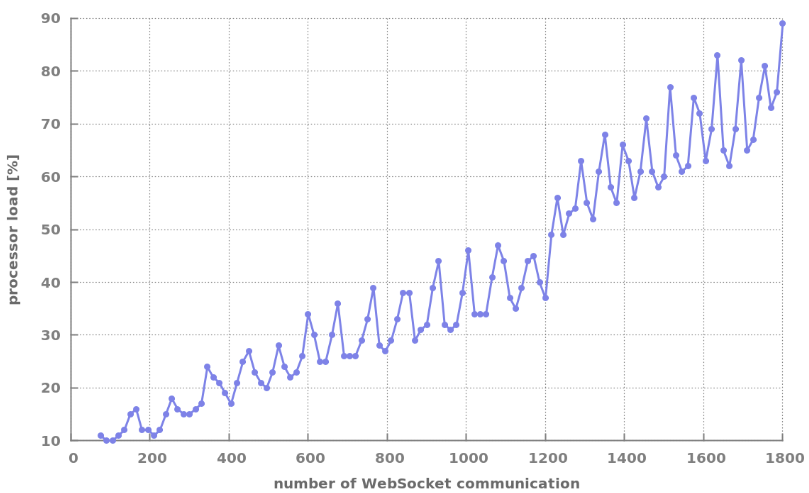
\includegraphics[width=\textwidth]{./Figures/1_client.png}
		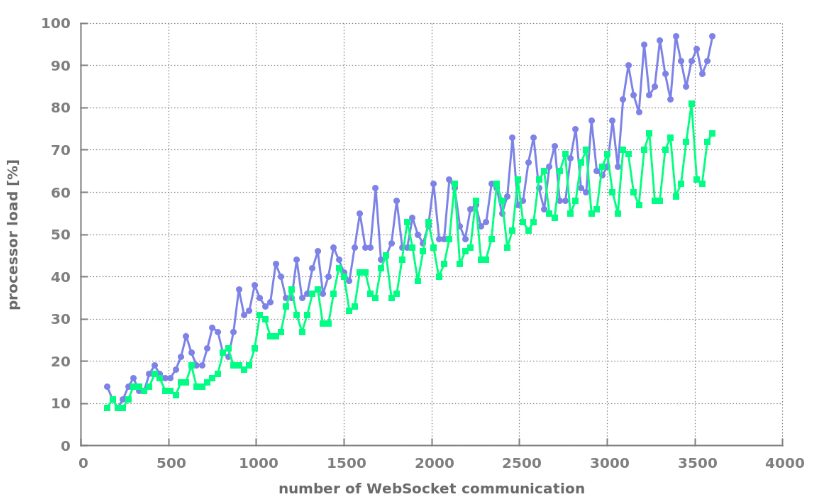
\includegraphics[width=\textwidth]{./Figures/2_client.png}
	\caption[1+2_client]{client throughout}
	\label{fig:1+2_client}
\end{figure}


From figure \ref{fig:1+2_client} can be inferred that the client
implementation works flawlessly. Adding a second core enables twice as much
communication  to be established.

\subsection{browser testing}

As mentionned in appendix \ref{fig:index_script}, by opering minor changes in
the \texttt{index.html} file, the browser can be configured to display in real
time the number of pings received by a particular worker. If the experiment is
running locally, typing \texttt{localhost:8080} in the url will link the
browser to one worker.\\

\begin{figure}[H]
	\centering
		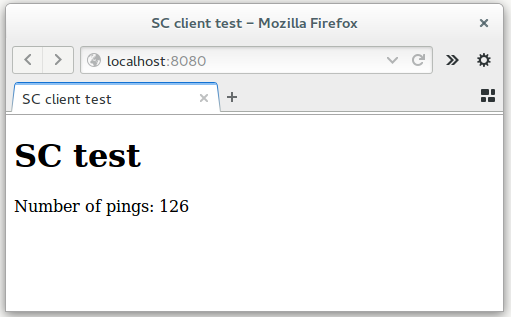
\includegraphics[width=0.9\textwidth]{./Figures/browser.png}
	\caption[browser]{Browser connection to SocketCluster}
	\label{fig:browser}
\end{figure}

By doing so we can embody a user connected to our WebSocket server and have a
better idea of the reactivity of the server.

% --------------
% second section
% --------------

\section{Comparaison with engine.io}

SocketCluster has been created to ease the creation of multi - core WebSocket
server. Logicaly the first experiment carried out on the server was to compare
a WebSocket to a traditionnal Engine.io server. 

Engine.io and SocketCluster codes can be found in appendix \ref{SocketCluster} and \ref{engine}. 

\begin{center}
  \begin{tabular}{ | l | l |}
  \hline
  \multicolumn{2}{|c|}{Parameters} \\
  \hline
    Instance type &  amazon ec2 m3.2xlarge\\ 
    Experiment time & 60 s \\
    Number of new communication created at each iteration & 20 \\
    Client creation period & 1 s \\
    Type of ping & random number \\ 
    Ping period & 2.5 s \\ 
    Number if clients & 2 \\
  \hline
  \end{tabular}
\end{center}


\begin{figure}[H]
	\centering
		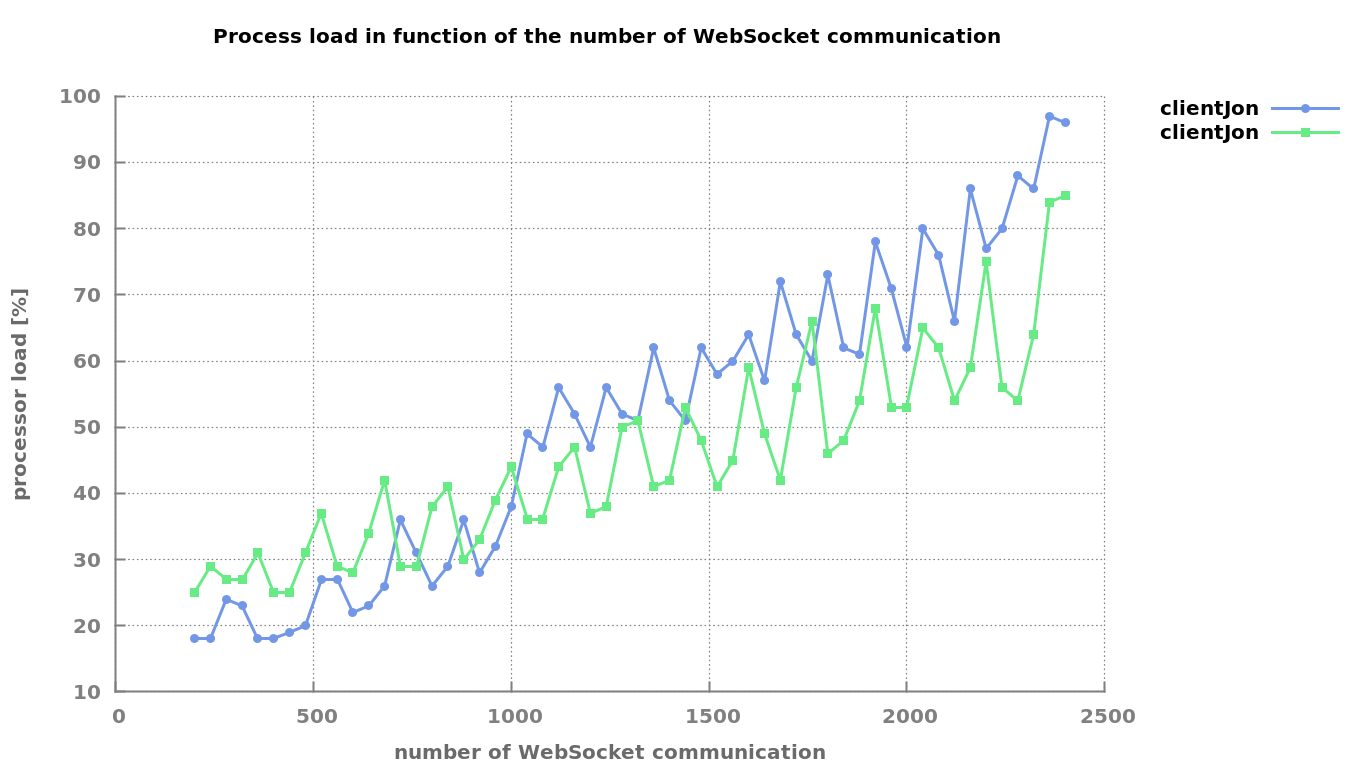
\includegraphics[width=\textwidth]{./Figures/WS_client_comparaison.png}
		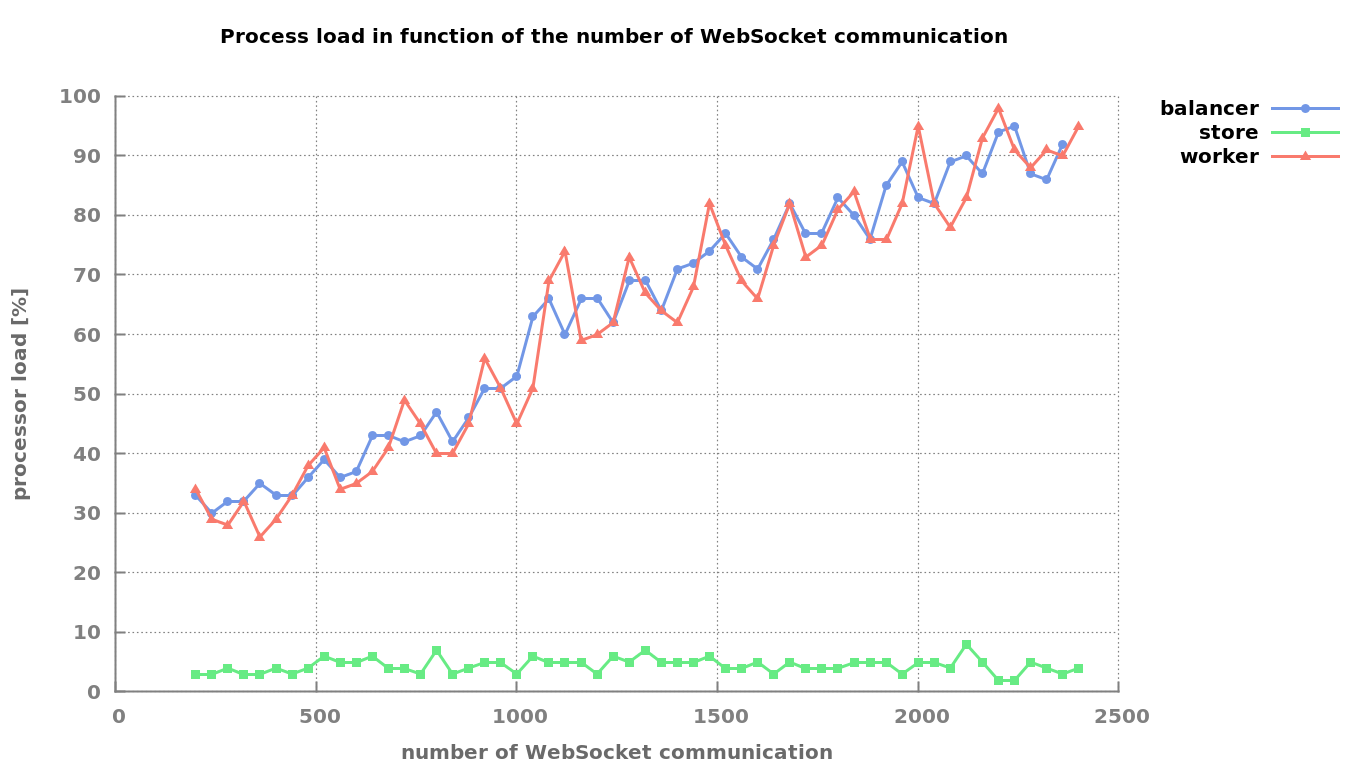
\includegraphics[width=\textwidth]{./Figures/WS_server_comparaison.png}
	\caption[WS_comparaison]{WebSocket implementation}
	\label{fig:WS_comparaison}
\end{figure}

In this experience, two clients are used to achieve a maximum of 2400 WebSocket
communications.  The server was configured to use one storage, one load
balancer and one worker. While the store processor is quite idle, the two other
processors on the other hand are almost used at full capacity.

\begin{figure}[H]
	\centering
		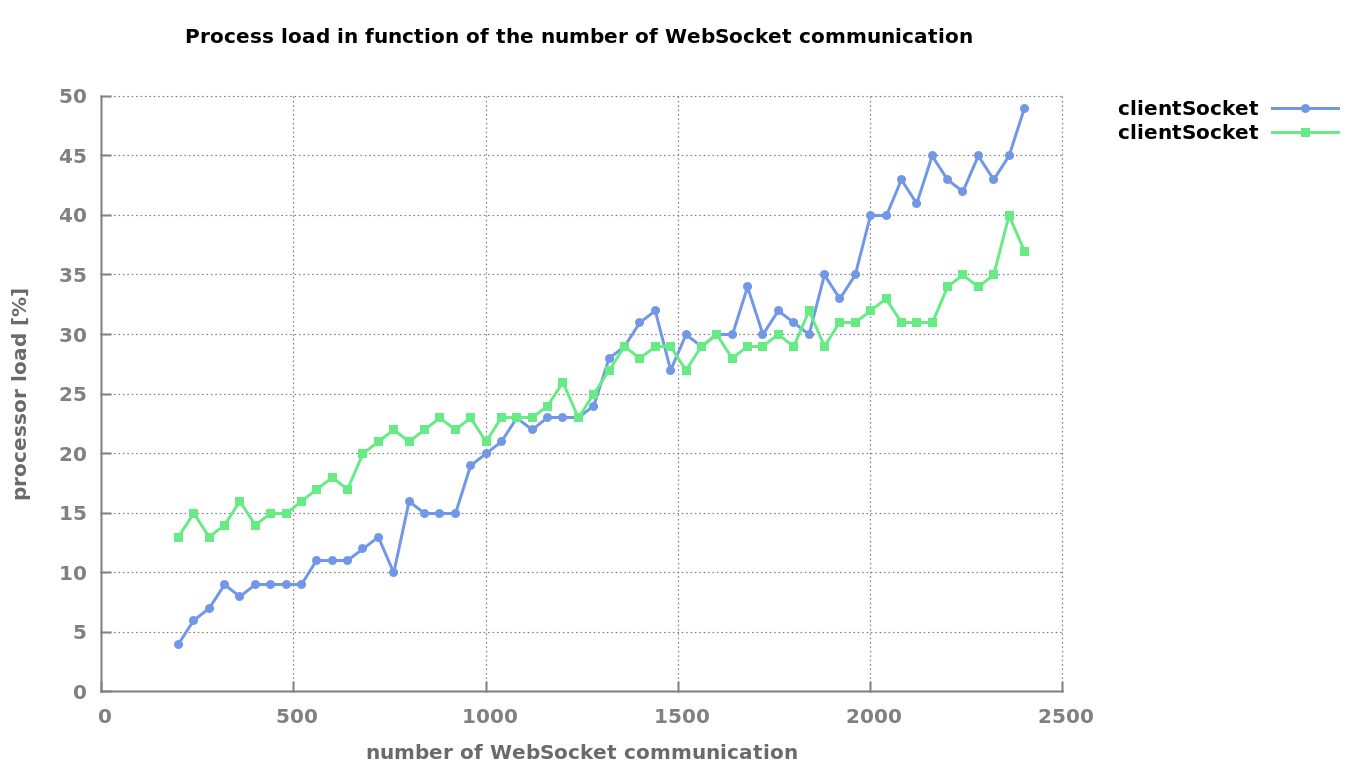
\includegraphics[width=\textwidth]{./Figures/engine_client_comparaison.png}
		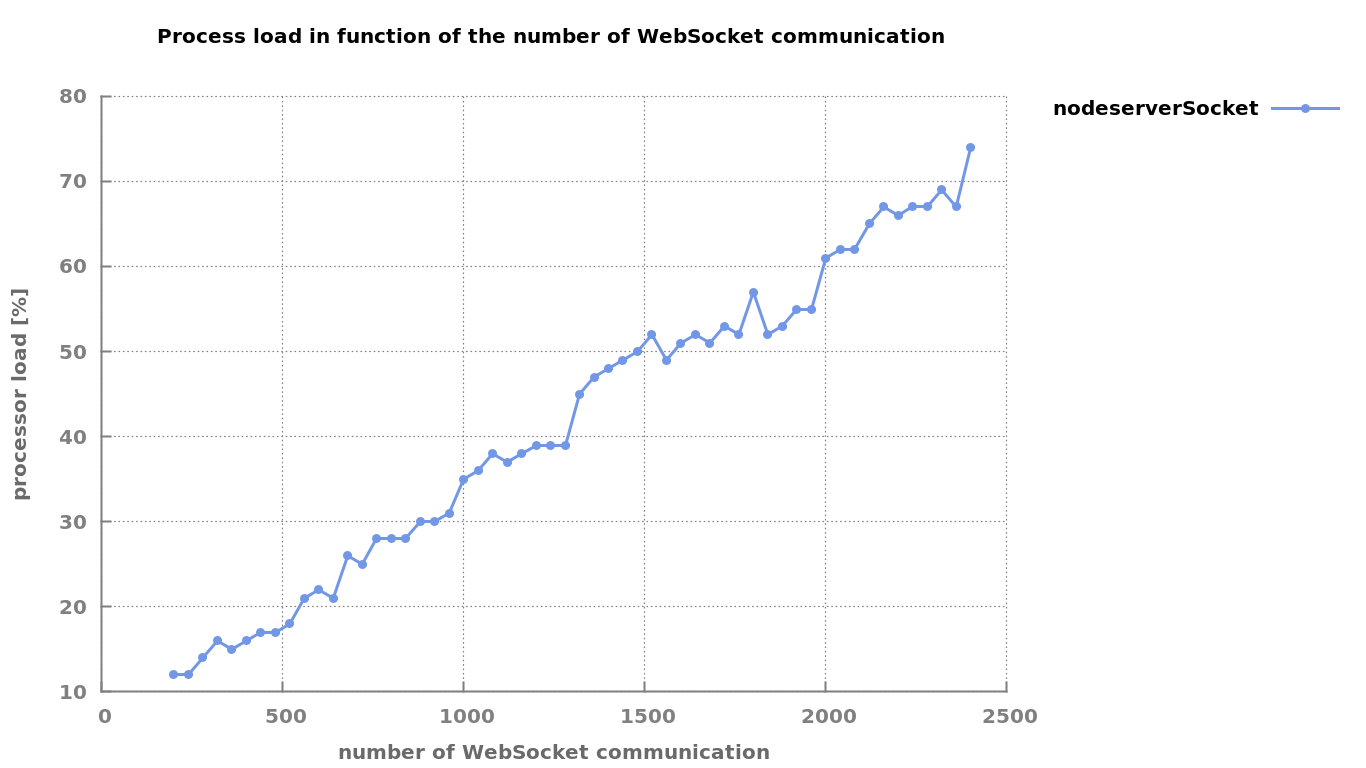
\includegraphics[width=\textwidth]{./Figures/engine_server_comparaison.png}
	\caption[engine_comparaison]{Engine.io implementation}
	\label{fig:engine_comparaison}
\end{figure}

Surprisingly, pure engine.io implementation seems to be more efficient. Clients
are hitting a maximum of 50\% processor usage compared to 90\% for WebSockets.

On the server side also, engine.io processor peaks at 75\% compared to almost
100\% for WebSockets. Also even if both code have been deployed on similar
virtual machines: \texttt{amazon ec2 m3.2xlarge} the engine.io server is
running only only on one core compared to three for SocketCluster (one storage,
one load balancer and one worker)

An interesting experiment worth mentionning, is to try to use SocketCluster on
one core.

% -------------
% Third section
% -------------

\section{SocketCluster context switching}
\section{}

This experiment's goal is to see the influence of additionnal worker and load balancer.

\textbf{Client code}

The client code used in all this part is the same. Two clients are used to
produce a maximum of 2400 WebSocket communications.


\begin{center}
  \begin{tabular}{ | l | l |}
  \hline
  \multicolumn{2}{|c|}{Parameters} \\
  \hline
    Instance type &  amazon ec2 m3.2xlarge\\ 
    Experiment time & 60 s \\
    Number of new communication created at each iteration & 20 \\
    Client creation period & 1 s \\
    Type of ping & random number \\ 
    Ping period & 2.5 s \\ 
    Number if clients & 2 \\
  \hline
  \end{tabular}
\end{center}


\begin{figure}[H]
	\centering
		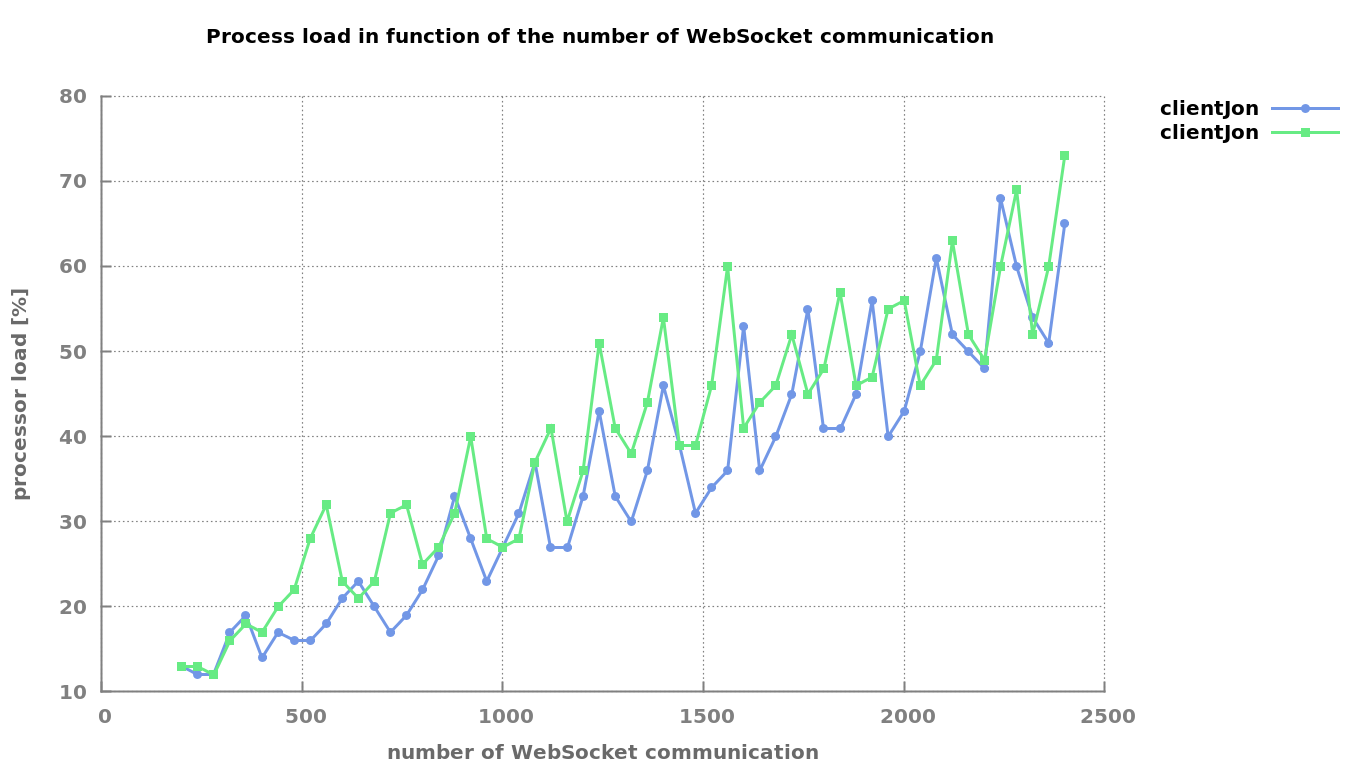
\includegraphics[width=\textwidth]{./Figures/WS_client_rising.png}
	\caption[WS_client_rising]{client code}
	\label{fig:WS_client_rising}
\end{figure}

\begin{figure}[H]
	\centering
		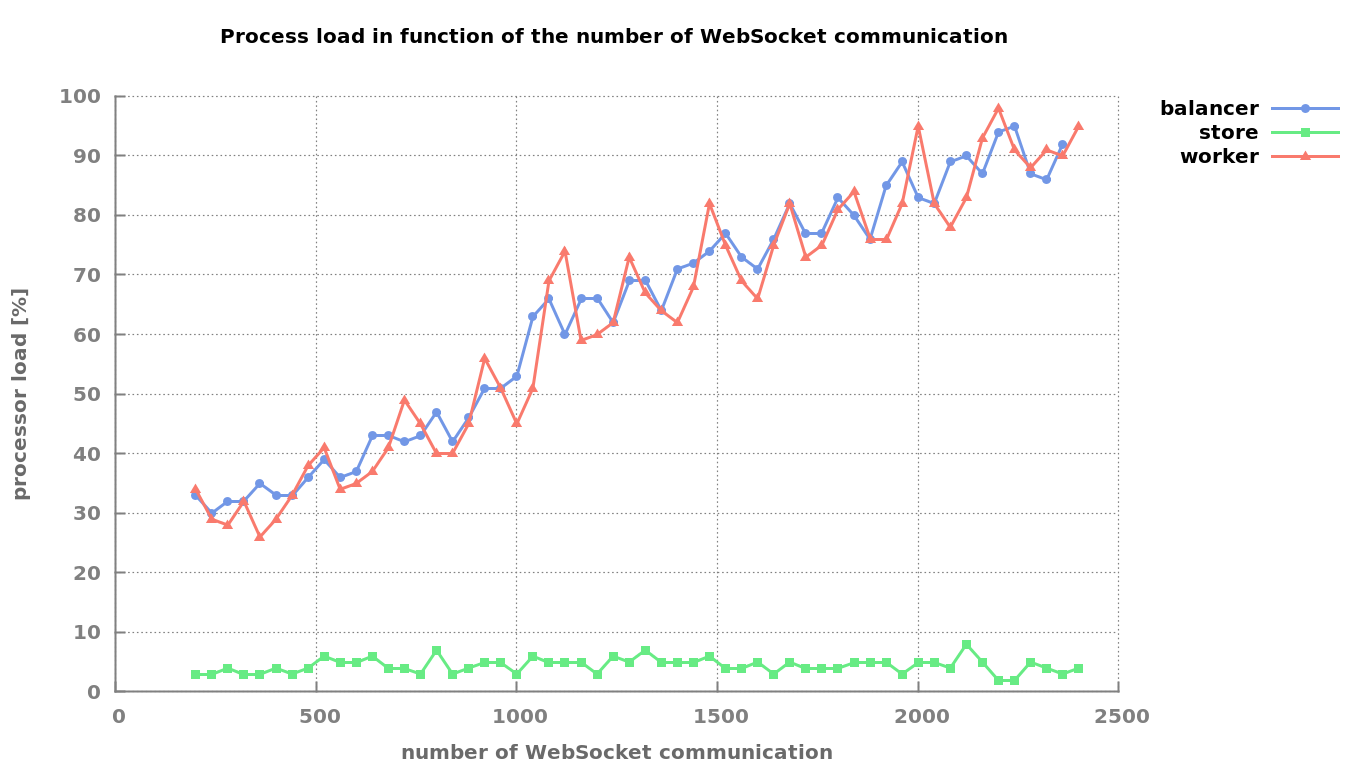
\includegraphics[width=\textwidth]{./Figures/WS_server_1rising.png}
	\caption[WS_server_1rising]{Server with 3 cores}
	\label{fig:WS_server_1rising}
\end{figure}

figure \ref{fig:WS_server_1rising} clearly shows the worker and loadbalancer
cores are almost to the full extent. In order to handle more communication more
cores should be added. 

\begin{figure}[H]
	\centering
		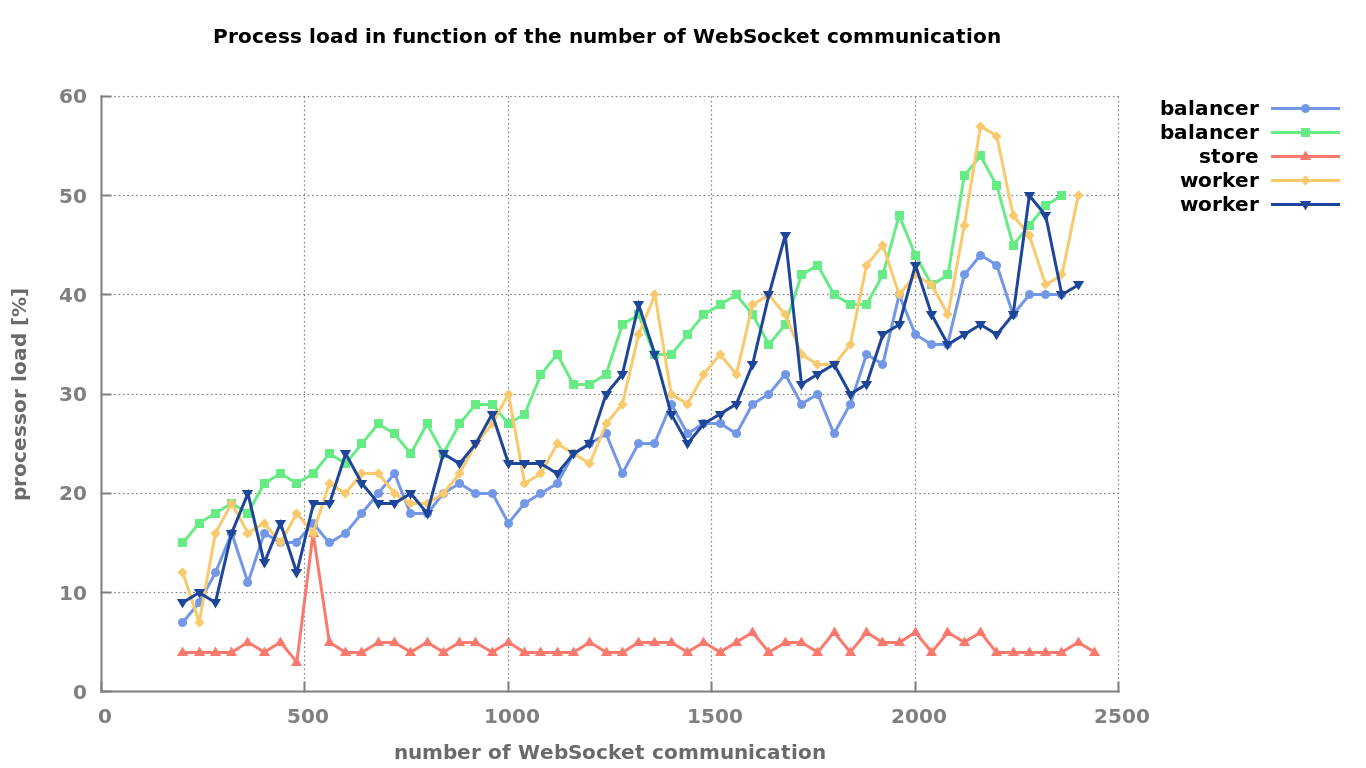
\includegraphics[width=\textwidth]{./Figures/WS_server_2rising.png}
	\caption[WS_server_2rising]{server with 5 cores}
	\label{fig:WS_server_2rising}
\end{figure}

In this experiment two more cores have been thrown to work. Load balancers and
workers nicely balance the work between themselves and the maximum load drops to 50\%.

\begin{figure}[H]
	\centering
		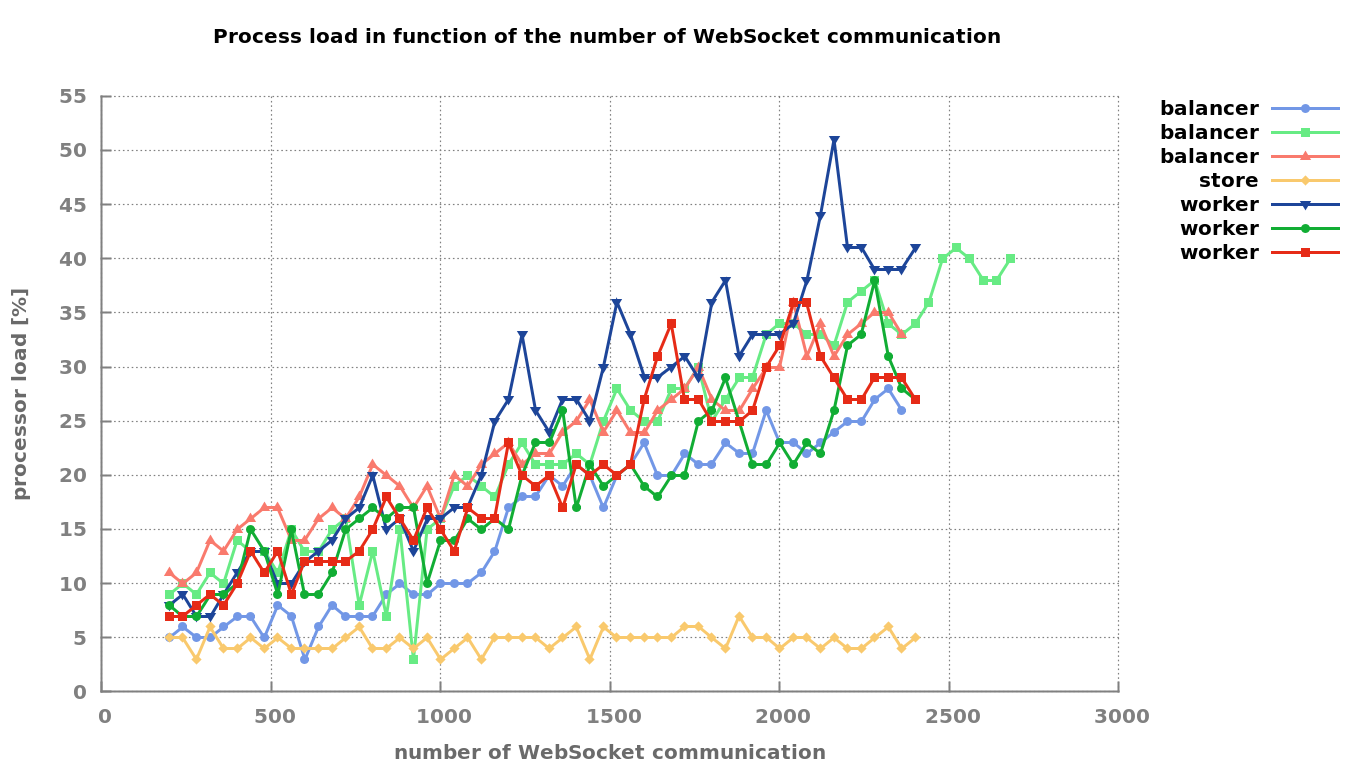
\includegraphics[width=\textwidth]{./Figures/WS_server_3rising.png}
	\caption[WS_server_3rising]{server with 7 cores}
	\label{fig:WS_server_3rising}
\end{figure}

this last test is less conclusive. With a total of 3 cores for load balancers
and three for workers the processors load varies between 30\% and 50\%
depending on the task.

B] section most influence frequence pings / size message / number communications

c] General rule

load balancer / store / worker
